\documentclass[11pt,oneside]{book}
\usepackage{underscore}
\usepackage[margin=1in]{geometry}
\usepackage{xcolor}
\usepackage{graphicx}
\usepackage{longtable,booktabs,array}
\usepackage{fancyvrb}
\usepackage[hidelinks]{hyperref}
\providecommand{\tightlist}{\setlength{\itemsep}{0pt}\setlength{\parskip}{0pt}}
\ifdefined\darkmode\pagecolor[HTML]{091117}\color[HTML]{F0EDE4}\fi
\graphicspath{{../renders/}{../reports/browser/}}
\title{PaxosKV\\[1ex]\large A complete LeanFM worked example}
\author{Project team}
\date{\today}
\begin{document}
\frontmatter
\maketitle
\tableofcontents
\mainmatter

\chapter{What this project is}
PaxosKV is a key/value database replicated across three Paxos replicas, with
a one-page web front end. Two browser sessions can write at the same time;
each write is acknowledged only after two replicas have durably stored it,
and every listing shows one committed prefix of the log.

It is the smallest complete example of the LeanFM method: one book (this
one), typed requirements in \texttt{spec/Requirements.lean} and
\texttt{spec/Requirements.proto}, an implementation mapping in
\texttt{spec/Implementation.lean}, Go source in \texttt{source/}, views
derived from the requirements in \texttt{renders/}, and evidence from real
runs in \texttt{reports/}. Everything the project owns lives under this one
directory.

\section{Reproducing everything}
From the project root, with the LeanFM installation built (\texttt{make build}
two directories up):
\begin{Verbatim}
make spec-check     # compile and validate the Lean specification
make views          # regenerate renders/ from the requirements
make app-check      # go vet, go test -race
make run            # three replicas + web app on 127.0.0.1:8082
make browser-check  # (second terminal) two concurrent browser sessions
make book           # this book, light and dark
\end{Verbatim}
Replica data lives in \texttt{.cache/data/} and survives restarts;
\texttt{make -C source clean-data} deletes it.

\chapter{Requirements}
\hypertarget{boundary-and-assumptions}{%
\section{Boundary and assumptions}\label{boundary-and-assumptions}}

The Paxos participant is \texttt{KVReplica}, instantiated as one
homogeneous cluster of exactly three members: \texttt{kv-0},
\texttt{kv-1}, and \texttt{kv-2}. \texttt{Browser} and \texttt{WebApp}
are actors but are not Paxos participants. Two independent browser
sessions may have tasks in flight concurrently.

The confirmed availability premise means that at every modeled instant
at least two replicas are running, all replicas can reach one another
while running, and each can reach its durable storage. This gives a live
majority. Persistence additionally requires an acceptor to fsync its
accepted ballot, slot, key, and value before sending \texttt{Accepted};
the web response is not successful until a quorum of two durable
acceptances exists. A restarted replica recovers its accepted log before
participating. If all three replicas stop, the service is unavailable
rather than forgetful: after restart, quorum recovery reconstructs the
committed log from durable acceptor state before reads or writes resume.

The confirmed conflict rule is last-committed-slot-wins: if the two
browser sessions write the same key concurrently, the leader assigns
distinct Paxos log slots and the value in the later committed slot is
displayed.

\hypertarget{related-grammar-set}{%
\section{Related grammar set}\label{related-grammar-set}}

\begin{verbatim}
project paxos_kv ::=
  repeat(quorum_write || linearizable_list || recover_replica)

quorum_write ::=
  Browser.Put(key, value, session, request_id) ;
  WebApp.Propose(key, value, session, request_id) ;
  Leader.Assign(ballot, slot) ;
  parallel(
    Replica.Accept(ballot, slot, key, value) ;
    Replica.Accept(ballot, slot, key, value) ;
    Replica.Accept(ballot, slot, key, value)
  ) ;
  mOfN(2, Replica.DurableAccepted(ballot, slot)) ;
  Leader.Commit(ballot, slot, key, value) ;
  WebApp.PutSucceeded(key, value, slot) ;
  ref(linearizable_list)

linearizable_list ::=
  Browser.List(session, request_id) ;
  WebApp.ReadBarrier(ballot) ;
  mOfN(2, Replica.ReadBarrierAck(ballot, committed_slot)) ;
  Leader.Snapshot(committed_slot, entries) ;
  WebApp.ListSucceeded(committed_slot, entries)

recover_replica ::=
  Replica.Unavailable(instance) ;
  Replica.Restarted(instance) ;
  Replica.RecoverAcceptedLog(instance) ;
  Replica.CatchUp(committed_slot) ;
  Replica.Available(instance)
\end{verbatim}

The notation above is intentionally behavioral. An implementation may
use a stable Multi-Paxos leader, but leader election and ballot changes
must remain observable whenever leadership changes.

\hypertarget{two-session-interaction-projection}{%
\section{Two-session interaction
projection}\label{two-session-interaction-projection}}

This is the interaction structure to be generated from the grammar. The
two browser branches are incomparable until the leader assigns slots;
either may arrive first.

\begin{verbatim}
Browser A      Browser B        WebApp          KV leader       KV followers
    | PUT a=1      |               |                 |                 |
    |------------->|               |                 |                 |
    |               | PUT b=2      |                 |                 |
    |               |------------->|                 |                 |
    |               |               | propose A      |                 |
    |               |               |--------------->|                 |
    |               |               | propose B      |                 |
    |               |               |--------------->|                 |
    |               |               |          assign slots s,s+1      |
    |               |               |                 | accept/fsync -->|
    |               |               |                 |<-- accepted (2) |
    |               |               |<-- commit A ----|                 |
    |<-- success + current list ----|                 |                 |
    |               |               |                 | accept/fsync -->|
    |               |               |                 |<-- accepted (2) |
    |               |               |<-- commit B ----|                 |
    |               |<-- success + current list ------|                 |
\end{verbatim}

The durable event representation must keep separate
\texttt{(session,\ scenario)} keys and use \texttt{priorIds} to record
immediate predecessor order. \texttt{priorIds\ =\ {[}{]}} means that an
event is a minimal (first) event in the scenario. If several events have
no predecessor, they are mutually unordered and may proceed in parallel.
A singleton list is the ordinary prior-event link; a list with several
IDs is a join. These links are ordering backpointers, not claims of
causation. Event file line order must not serialize otherwise unordered
browser requests.

\hypertarget{observable-safety-and-progress-obligations}{%
\section{Observable safety and progress
obligations}\label{observable-safety-and-progress-obligations}}

\begin{itemize}
\tightlist
\item
  A successful PUT necessarily has two prior \texttt{DurableAccepted}
  observations for the same ballot, slot, key, and value.
\item
  No two different values are committed for the same log slot.
\item
  Every committed slot remains present after any one replica is
  unavailable.
\item
  A list result reflects one committed prefix selected after a quorum
  read barrier; it does not combine entries from different prefixes.
\item
  With two mutually reachable durable replicas and a leader eventually
  chosen, every accepted browser request eventually succeeds or returns
  an explicit error.
\item
  Replica unavailability, leadership loss, retry, rejection, and
  recovery are visible outcomes rather than hidden timeouts.
\item
  At most three replica instances exist, all implementing the same
  \texttt{KVReplica} actor specification.
\end{itemize}

\hypertarget{prompt-derived-outputs}{%
\section{Prompt-derived outputs}\label{prompt-derived-outputs}}

\begin{description}
\item[\texttt{paxos.write.interaction}] (interaction diagram) How does a browser write become persistent? \emph{Reducer:} Partition write events by \texttt{(session,request\_id)} and render quorum branches in \texttt{priorIds} order, with typed message fields in each node
\item[\texttt{paxos.write.state\_machine}] (state machine) Which observable write states and failure exits exist? \emph{Reducer:} Render residuals of \texttt{quorum\_write}
\item[\texttt{paxos.list.interaction}] (interaction diagram) How is the complete key/value listing made linearizable? \emph{Reducer:} Render list and read-barrier events by \texttt{(session,request\_id)}
\item[\texttt{paxos.list.state\_machine}] (state machine) Which observable list states and failure exits exist? \emph{Reducer:} Render residuals of \texttt{linearizable\_list}
\item[\texttt{paxos.concurrent.order}] (prior-pointer graph) Can two browser sessions access the app concurrently? \emph{Reducer:} Render incomparable request branches, slot assignment, quorum joins, and responses
\item[\texttt{paxos.commit\_latency}] (2D function) How does write latency change with concurrent browser sessions? \emph{Reducer:} Pair PUT start to success/error by prior ID; x=max concurrent sessions, y=latency milliseconds
\item[\texttt{paxos.quorum\_size}] (scalar and histogram) Did every acknowledged write have a durable majority? \emph{Reducer:} Count distinct accepting replica instances per committed slot
\item[\texttt{paxos.replica\_availability}] (line) Were at least two replicas available throughout the observation window? \emph{Reducer:} Sweep \texttt{Unavailable}/\texttt{Available} intervals and plot available replica count over monotonic time
\item[\texttt{paxos.recovery\_lag}] (2D function) How far behind is a restarting replica? \emph{Reducer:} x=time since restart; y=leader committed slot minus replica applied slot
\item[\texttt{paxos.outcomes}] (pie/histogram) What happened to browser PUT and list requests? \emph{Reducer:} Count success, explicit rejection, timeout/censored, and leadership-loss outcomes
\end{description}


Numeric reductions use these stable output IDs at \texttt{/metrics}.
Every diagram, state machine, and chart is derived from the accepted
grammar and events rather than maintained as a second specification.

\hypertarget{web-behavior}{%
\section{Web behavior}\label{web-behavior}}

The page contains a string \texttt{key} input, a string \texttt{value}
input, and a submit action. Below the form it renders the linearizable
listing of all committed key/value pairs. After a successful write the
initiating session receives a page containing a listing at least as new
as its committed write. The other browser session observes that write on
its next list operation; server push is not currently required.

There is no authentication and no delete operation. Keys are nonempty
UTF-8 strings of at most 128 encoded bytes. Values are UTF-8 strings of
at most 4096 encoded bytes. The database holds at most 10,000 distinct
keys and supports at least two browser sessions with requests in flight
concurrently. Invalid or capacity-exceeding writes return explicit
errors without changing the committed log. Each successful submission
returns a listing containing at least that committed write.


\chapter{Derived views}
Every figure in this chapter is generated by \texttt{spec/Views.lean} from
\texttt{Project.Requirements.requirements}; none is drawn by hand.

\begin{figure}[htbp]\centering
\includegraphics[width=\textwidth,height=0.8\textheight,keepaspectratio]{quorum-write.pdf}
\caption{Task \texttt{quorum\_write}: states and transitions.}
\end{figure}

\begin{figure}[htbp]\centering
\includegraphics[width=0.7\textwidth,height=0.8\textheight,keepaspectratio]{quorum-write-messages.pdf}
\caption{One concrete quorum write as a prior-pointer graph. The two
\texttt{Promise} events fork from \texttt{Prepare}; \texttt{Accept} and
\texttt{Commit} are two-of-three joins.}
\end{figure}

\begin{figure}[htbp]\centering
\includegraphics[width=\textwidth,height=0.45\textheight,keepaspectratio]{linearizable-list.pdf}
\caption{Task \texttt{linearizable\_list}.}
\end{figure}

\begin{figure}[htbp]\centering
\includegraphics[width=0.8\textwidth,height=0.45\textheight,keepaspectratio]{recover-replica.pdf}
\caption{Task \texttt{recover\_replica}.}
\end{figure}

\chapter{Implementation}
This chapter maps the requirements to an implementation. It does not
change their observable meaning.


\hypertarget{target-and-processes}{%
\section{Target and processes}\label{target-and-processes}}

\begin{itemize}
\tightlist
\item
  Target language: Go.
\item
  One \texttt{paxos-kv} executable with subcommands \texttt{web} and
  \texttt{replica}.
\item
  One WebApp process and three independently started replica processes.
\item
  Replica IDs and addresses are supplied explicitly; membership is fixed
  at \texttt{kv-0}, \texttt{kv-1}, and \texttt{kv-2}.
\item
  Browser traffic uses HTTP. Replica protocol traffic uses
  length-delimited protobuf messages over TCP connections.
\end{itemize}

\hypertarget{durable-state}{%
\section{Durable state}\label{durable-state}}

Each replica owns a separate data directory containing an append-only
accepted log and a small metadata file for the highest promised ballot.
Every update is written to a temporary record, flushed with
\texttt{fsync}, and atomically made visible before
\texttt{DurableAccepted} is sent. Recovery scans and validates the log,
truncates only an incomplete final record, and reconstructs accepted
slots. No process shares a replica data directory.

The leader records commit decisions durably. On startup or leadership
change it runs Paxos recovery against a quorum before accepting HTTP
work, choosing the accepted value with the highest ballot for each slot
and filling any gaps.

\hypertarget{consensus-and-reads}{%
\section{Consensus and reads}\label{consensus-and-reads}}

\begin{itemize}
\tightlist
\item
  Stable-leader Multi-Paxos assigns monotonically increasing log slots.
\item
  Ballots are ordered pairs \texttt{(counter,\ replica\_id)}.
\item
  A candidate must receive promises from two replicas before becoming
  leader.
\item
  A value is committed after two distinct replicas have durably accepted
  the identical \texttt{(ballot,\ slot,\ key,\ value)} tuple.
\item
  Repeated messages are idempotent by \texttt{(ballot,\ slot)} and
  browser \texttt{(session\_id,\ request\_id)}.
\item
  The materialized key/value map applies committed slots in increasing
  order; this implements last-committed-slot-wins.
\item
  A list request uses a quorum read barrier and returns one applied
  committed prefix. A successful PUT waits until its slot is applied,
  then obtains the listing from a prefix at least that new.
\end{itemize}

\hypertarget{web-application}{%
\section{Web application}\label{web-application}}

\begin{itemize}
\tightlist
\item
  \texttt{GET\ /} obtains a linearizable listing and renders the form
  followed by the sorted key/value table.
\item
  \texttt{POST\ /put} accepts form fields \texttt{key} and
  \texttt{value}, validates encoded byte limits, submits the write, and
  renders the resulting listing.
\item
  A secure random cookie supplies \texttt{session\_id}; every request
  gets a unique \texttt{request\_id}.
\item
  HTML is escaped. Request bodies, response bodies, and internal queues
  are bounded. Two browser sessions may progress concurrently.
\item
  Failures return an explicit page and appropriate HTTP status; they
  never display an uncommitted value as successful.
\end{itemize}

\hypertarget{resource-choices}{%
\section{Resource choices}\label{resource-choices}}

\begin{itemize}
\tightlist
\item
  Web request body: 8 KiB maximum.
\item
  WebApp: 64 in-flight requests and a bounded 128-item submission queue.
\item
  Each replica: bounded 256-message inbound queue and 64 simultaneous
  peer operations.
\item
  Database: 10,000 distinct keys, with limits enforced before proposal.
\item
  Timeouts cancel a client attempt but do not erase a value already
  accepted; retries use the same request ID and discover the committed
  result.
\end{itemize}

\hypertarget{observability}{%
\section{Observability}\label{observability}}

Every protocol transition is meant to emit the LeanFM event envelope with
event ID, repeated predecessor IDs, browser session, task/request ID,
concrete source and destination replica IDs, monotonic time, and
protobuf atom. \texttt{/metrics} exports commit latency, quorum size,
available replica count, recovery lag, request outcomes, queue depth,
and memory headroom under the accepted output IDs. Logs include ballot
and slot but never unescaped HTML.

\hypertarget{generated-source-layout}{%
\section{Generated source layout}\label{generated-source-layout}}

\begin{verbatim}
source/Makefile                       build, run, stop, test
source/runtime.py                     Runtime actor (supervisor)
source/browser_check.py               two-session browser check
source/cmd/paxos-kv/main.go           replica and web subcommands
source/internal/web/app.go            WebApp and Browser bindings
source/internal/paxos/node.go         KVReplica: Multi-Paxos and recovery
source/internal/paxos/storage.go      fsynced accepted log
source/internal/protocol/             wire Envelope (protobuf)
source/internal/metrics/metrics.go    /metrics
source/internal/trace/events.go       events/kv-N.jsonl
source/web/templates/index.html       the page
source/traceability.json              requirement -> file map
\end{verbatim}

\hypertarget{conformance-tests}{%
\section{Conformance tests}\label{conformance-tests}}

\begin{itemize}
\tightlist
\item
  Two browser sessions write different keys concurrently and both
  listings converge to the same committed map.
\item
  Two sessions write one key concurrently; the later committed slot
  wins.
\item
  Every HTTP success has two prior durable acceptances from distinct
  replicas.
\item
  Stop any one replica during writes; the other two continue and the
  stopped replica catches up after restart.
\item
  Stop all replicas after acknowledged writes; restart two and recover
  every acknowledged value before serving.
\item
  Corrupt or truncate the final log record and verify safe recovery
  without inventing a commit.
\item
  Reject oversized, empty-key, and 10,001st-key writes without mutation.
\item
  Reject conflicting values for one slot, stale ballots, malformed
  protobuf, and illegal trace order.
\item
  Exercise full queues, timeouts, idempotent retries, and HTML escaping.
\end{itemize}


The observability section above is the target. Today the replicas emit
only terminal events; see the Known gaps chapter.

\section{Runtime}
\texttt{source/runtime.py} is the \texttt{Runtime} actor: it starts
\texttt{kv-0}, \texttt{kv-1}, \texttt{kv-2} on ports 9100--9102 and the web
app on 8082, records its own process identity, and stops only that process.
Each replica appends its observed events to \texttt{events/kv-N.jsonl}.

\chapter{Running it}
\texttt{source/browser\_check.py} opens two independent browser sessions
against a running deployment. Session A writes \texttt{color=blue} while
session B writes \texttt{shape=circle} concurrently; A then overwrites
\texttt{color=green}. Both sessions then list the database. The screenshots
below are produced by that script; \texttt{reports/browser/browser-check.json}
records the rows each session saw.

\begin{figure}[htbp]\centering
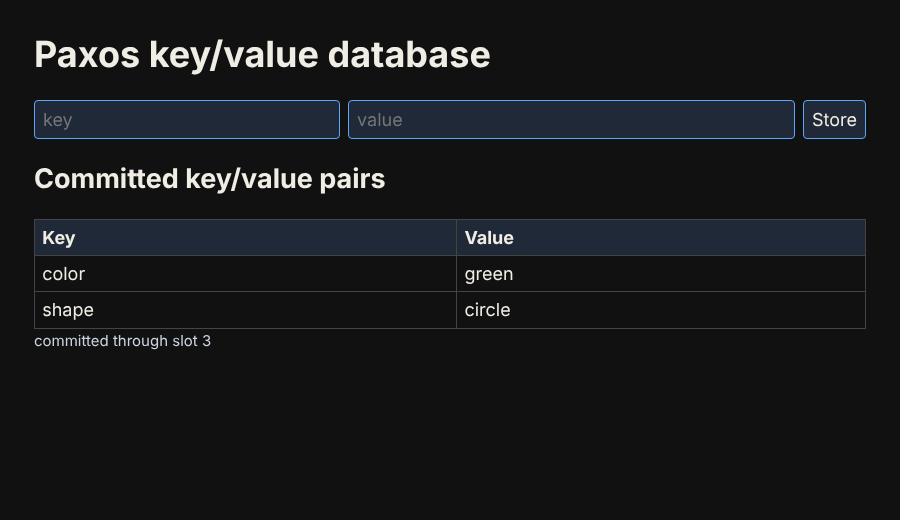
\includegraphics[width=0.48\textwidth]{session-a.png}\hfill
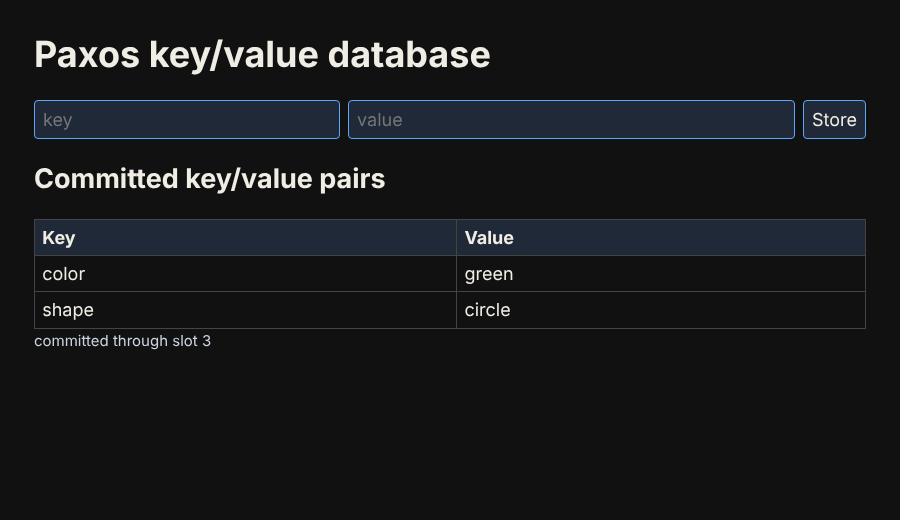
\includegraphics[width=0.48\textwidth]{session-b.png}
\caption{Session A (left) and session B (right) after the writes. Both show
the same committed map; the later slot for \texttt{color} wins.}
\end{figure}

\chapter{Known gaps}
This example runs end to end, but it does not yet close the loop from a
running system back to the checker. These are the open items, in the order
they should be fixed:
\begin{enumerate}
\item The protobuf message types in \texttt{spec/Requirements.proto} have no
  fields; the replicas send one generic \texttt{Envelope}. The typed messages
  in the requirements should become the wire format.
\item Replicas log only terminal events (\texttt{PutSucceeded},
  \texttt{ListSucceeded}) and record no \texttt{priorIds}. Every send and
  receive in the grammar should be logged with its predecessors, so a run
  can be replayed through \texttt{check\_trace} and the CTL checker.
\item The interaction diagram for a run should then be drawn from
  \texttt{events/} rather than from the hand-written example scenario.
\item The requirements declare three \texttt{WebApp} instances; the runtime
  starts one.
\item Go tests cover envelope round trips and truncated frames, not message
  loss, duplication, delay or reordering.
\end{enumerate}
\end{document}
